%!TEX root = max_main.tex
\section{Lecture 12: Coordinate Descent}
\subsection{Why Coordinate Descent?}
There are many classes of functions for which it is very cheap 
to compute directional derivatives along the standard basis vectors
$e_i, i \in [n]$.
%
For example, 
%
\begin{eqnarray}
f(x) = \|x\|^2 \text{ or } f(x) = \|x\|_1
\end{eqnarray}
%
This is especially true of common regularizers, 
%
which often take the form 
\begin{eqnarray}
R(x) = \sum_{i=1}^n R_i(x_i) \ .
\end{eqnarray}
%
More generally, many objectives and regularizes exhibit ``group sparsity''; that is,
%
\begin{eqnarray}
R(x) =  \sum_{j=1}^m R_{j}(x_{S_j})
\end{eqnarray}
where each $S_j, j \in [m]$ is a subsect of $[n]$, and similarly for $f(x)$.
%
Examples of functions with block decompositions and group sparsity include:
\begin{enumerate} 
	\item Group sparsity penalties;
	\item Regularizes of the form $R(U^\top x)$, where $R$ is
    coordinate-separable, and $U$ has sparse columns and so
    $(U^\top x) = u_i^\top x$ depends only on the nonzero entries of $U_i$;
	\item Neural networks, where the gradients with respect to some weights can be
    computed ``locally''; and
	\item ERM problems of the form 
    \begin{eqnarray}
    f(x) := \sum_{i=1}^n \phi_i(\langle w^{(i)} , x \rangle )
    \end{eqnarray}
    where $\phi_i: \R \to \R$, and $w^{(i)}$ is non-zero except in a few coordinates. 
\end{enumerate} 


\begin{figure}[t]
\centering

\definecolor{myblue}{RGB}{80,80,160}
\definecolor{mygreen}{RGB}{80,160,80}
\usetikzlibrary{positioning,chains,fit,shapes,calc}

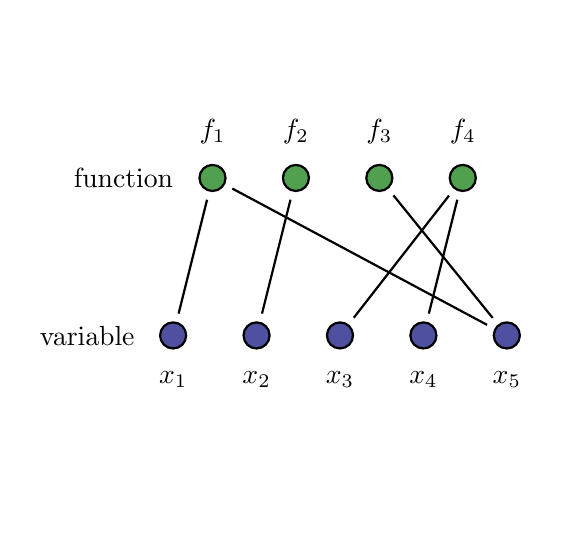
\begin{tikzpicture}[thick,
  every node/.style={draw,circle},
  fsnode/.style={fill=myblue},
  ssnode/.style={fill=mygreen},
  every fit/.style={draw=none},
  shorten >= 3pt,shorten <= 3pt
]

% Function
\begin{scope}[start chain=going right,node distance=7mm]
\foreach \i in {1,2,...,5}
  \node[fsnode,on chain] (x\i) [label=below: $x_\i$] {};
\end{scope}
\node [myblue,fit=(x1) (x5),label=left:variable] {};

% Coordinates
\begin{scope}[yshift=2cm,xshift=.5cm,start chain=going right,node distance=7mm]
\foreach \i in {1,2,...,4}
  \node[ssnode,on chain] (f\i) [label=above: $f_\i$] {};
\end{scope}
\node [mygreen,fit=(f1) (f4),label=left:function] {};

% Edges
\draw (x1) -- (f1);
\draw (x2) -- (f2);
\draw (x3) -- (f4);
\draw (x4) -- (f4);
\draw (x5) -- (f1);
\draw (x5) -- (f3);
\end{tikzpicture}
\vspace{-20pt}
\caption{
  Example of the bipartite graph between component functions
  $f_i, i \in [m]$ and variables $x_j, j \in [n]$ induced by the
  group sparsity structure of a function $f : \R^n \to \R^m$.
  An edge between $f_i$ and $x_j$ conveys that the $i$th component function
  depends on the $j$th coordinate of the input.
}
\end{figure}

\section{Coordinate Descent}
  Denote $\partial_i f= \frac{\partial f}{x_i}$.
  For each round $t = 1,2,\dots$, the coordinate descent algorithms
  chooses an index $i_t \in [n]$, and computes
	\begin{eqnarray}
	x_{t+1} = x_t - \eta_t\partial_{i_t}f(x_t) \cdot e_{i_t} \ .
	\end{eqnarray}
  This algorithm is a special case of stochastic gradient descent. For
	\begin{eqnarray}
    \E[x_{t+1} | x_t]
    &=& x_t - \eta_t \E [\partial_{i_t}f(x_t) \cdot e_{i_t}] \\
    &=& x_t - \frac{\eta_t}{n} \sum_{i=1}^n \partial_{i}f(x_t) \cdot e_i \\
    &=& x_t - \eta_t \nabla f(x_t) \ .
	\end{eqnarray}
	Recall the bound for SGD: If $\E[g_t] = \nabla f(x_t)$, then SGD with step size $\eta = \frac{1}{BR}$ satisfies
	\begin{eqnarray}
	\E[f(\frac{1}{T}\sum_{t=1}^T x_t)] - \min_{x \in \Omega}f(x) \le \frac{2 BR}{\sqrt{T}}
	\end{eqnarray}
	where $R^2$ is given by $\max_{x \in \Omega} \|x-x_1\|^2_2$ and $B = \max_{t}\E[\|g_t\|^2_2]$. In particular, if we set $g_t = n \partial_{x_{i_t}}f(x_t) \cdot e_{i_t}$, we compute that
	\begin{eqnarray}
    \E[\|g_t\|^2_2]
    = \frac{1}{n} \sum_{i=1}^n \|n\cdot \partial_{x_{i}}f(x_t) \cdot e_i\|^2_2
    = n \|\nabla f(x_t)\|^2_2 \ .
	\end{eqnarray}
	If we assume that $f$ is $L$-Lipschitz, we additionally have that 
	$\E[\|g_t\|^2] \le nL^2$.
  This implies the first result:
	\begin{proposition} Let $f$ be convex and $L$-Lipschitz on $\R^n$.
    Then coordinate descent with step size $\eta = \frac{1}{n R}$ has convergence rate 
	\begin{eqnarray}
	\E[f(\frac{1}{T}\sum_{t=1}^T x_t)] - \min_{x \in \Omega}f(x) \le 2LR\sqrt{n/T}
	\end{eqnarray}
	\end{proposition}
	\subsection{Importance Sampling}
	In the above, we decided on using the uniform distribution to sample a
  coordinate. But suppose we have more fine-grained information. In particular, what if we knew that we could bound $\sup_{x \in \Omega} \|\nabla f(x)_i\|_2 \le L_i$? An alternative might be to sample in a way to take $L_i$ into account. This motivates the ``importance sampled'' estimator of $\nabla f(x)$, given by
	\begin{eqnarray}
	g_t = \frac{1}{p_{i_t}} \cdot \partial_{i_t}f(x_{t}) \text{ where } i_t \sim
    \mathrm{Cat}(p_1,\dots,p_n) \ .
	\end{eqnarray}
	Note then that $\E[g_t] = \nabla f(x_t)$, but
	\begin{eqnarray}
    \E[\|g_t\|^2_2]
    &=& \sum_{i=1}^n (\partial_{i_t}f(x_{t}))^2/p_i^2\\
    &\le& \sum_{i=1}^n L_i^2/p_i^2
	\end{eqnarray}
	In this case, we can get rates 
	\begin{eqnarray}
	  \E[f(\frac{1}{T}\sum_{t=1}^T x_t)] - \min_{x \in \Omega}f(x)
    \le 2R\sqrt{1/T}\cdot \sqrt{\sum_{i=1}^n L_i^2/p_i^2}
	\end{eqnarray}
	In many cases, if the values of $L_i$ are heterogenous, we can optimize the values of $p_i$. 
	\subsection{Importance Sampling For Smooth Coordinate Descent}
	In this section, we consider coordinate descent with an \emph{biased}
  estimator of the gradient. Suppose that we have, for $x \in \R^n$
  and $\alpha \in \R$, the inequality
	\begin{eqnarray}
    |\partial_{x_i} f(x) - \partial_{x_i} f(x + \alpha e_i)|
    \le \beta_{i}|\alpha|
	\end{eqnarray}
	where $\beta_i$ are possibly heterogenous. Note that if that $f$ is twice-continuously differentiable, the above condition is equivalently to $\nabla^2_{ii}f(x) \le \beta_i$, or that $\mathrm{Diag}(\nabla^2 f(x)) \preceq \mathrm{diag}(\boldsymbol{\beta})$.  Define the distribution $p^\gamma$ via
	\begin{eqnarray}
	p^{\gamma}_i = \frac{\beta_i^{\gamma}}{\sum_{j=1}^n \beta_j^{\gamma}}
	\end{eqnarray}
	We consider gradient descent with the rule called $\mathrm{RCD}(\gamma)$
	\begin{eqnarray}\label{RCDgamma}
    x_{t+1} = x_t - \frac{1}{\beta_{i_t}} \cdot \partial_{i_t}(x_t) \cdot e_{i_t}, \text{ where } i_t \sim p^{\gamma}
	\end{eqnarray}
  Note that as $\gamma \to \infty$, coordinates with larger values of $\beta_i$
  will be selected more often.
	Also note that this is \emph{not generally} equivalent to SGD, because 
	\begin{eqnarray}
    \E\left[\frac{1}{\beta_{i_t}}\partial_{i_t}(x_t)e_i\right]
    = \frac{1}{\sum_{j=1}^n \beta_j^{\gamma}} \cdot \sum_{i=1}^n \beta_{i}^{\gamma - 1} \partial_i f(x_t)e_i
    = \frac{1}{\sum_{j=1}^n \beta_j^{\gamma}} \cdot \nabla f(x_t) \circ (\beta_i^{\gamma - 1})_{i \in [n]}
	\end{eqnarray}
	which is only a scaled version of $\nabla f(x_t)$ when $\gamma = 1$. Still, we can prove the following theorem:
	\begin{theorem}
  \label{thm:6.7}
  Define the weighted norms
	\begin{eqnarray}
	\|x\|_{[\gamma]}^2 := \sum_{i=1}^n x_i^2 \beta_i^\gamma \text{ and } \|x\|_{[\gamma]}^{*2} := \sum_{i=1}^n x_i^2 \beta_i^{-\gamma}
	\end{eqnarray}
	and note that the norms are dual to one another.
  We then have that the rule $\mathrm{RCD}(\gamma)$ produces iterates satisfying
	\begin{eqnarray}
	  \E[f(x_t) - \arg\min_{x \in \R^{n}} f(x)]
    \le \frac{2 R^2_{1-\gamma} \cdot \sum_{i=1}^n \beta_{i}^{\gamma}}{t-1}~,
	\end{eqnarray}
	where $R^2_{1-\gamma} = \sup_{x \in \R^n:f(x) \le f(x_1)} \|x - x^*\|_{[1 - \gamma]}$.
	\end{theorem}
	\begin{proof}
	Recall the inequality that for a general $\beta_g$-smooth convex function $g$, one has that
	\begin{eqnarray}
    g\left(u - \frac{1}{\beta_g}\nabla g(u)\right) - g(u)
    \le -\frac{1}{2\beta_g} \|\nabla g\|^2
	\end{eqnarray}
	Hence, considering the functions $g_i(u;x) = f(x + ue_i)$, we see that $\partial_i f(x) = g_i'(u;x)$, and thus $g_i$ is $\beta_i$ smooth. Hence, we have 
	\begin{eqnarray}
    f\left(x - \frac{1}{\beta_i}\nabla f(x)e_i\right) - f(x)
    = g_i(0 - \frac{1}{\beta_g}g_i'(0;x)) - g(0;x)
    \le -\frac{g_i'(u;x)^2}{2\beta_i} = - \frac{\partial_i f(x)^2}{2\beta_i} \ .
	\end{eqnarray}
	Hence, if $i~p^\gamma$, we have
	\begin{eqnarray}
	  \E[f(x - \frac{1}{\beta_i}\partial_i f(x)e_i) - f(x)]
    &\le& \sum_{i=1}^n p_i^\gamma \cdot - \frac{\partial_i f(x)^2}{2\beta_i}\\
	  &=& -\frac{1}{2\sum_{i=1}^n \beta_i^{\gamma}} \sum_{i=1}^n \beta^{\gamma - 1}\partial_i f(x)^2 \\
	  &=& -\frac{\|\nabla f(x)\|^{*2}_{[1-\gamma]})}{2\sum_{i=1}^n \beta_i^{\gamma}}
	\end{eqnarray}
	Hence, if we define $\delta_t = \E[f(x_t) - f(x^*)]$, we have that
	\begin{eqnarray}
	\delta_{t+1} - \delta_t \le -\frac{\|\nabla f(x_t)\|^{*2}_{[1-\gamma]}}{2\sum_{i=1}^n \beta_i^{\gamma}} 
	\end{eqnarray}
	Moreover, with probability $1$, one also has that $f(x_{t+1}) \le f(x_t)$, by the above. We now continue with the regular proof of smooth gradient descent. Note that
	\begin{eqnarray*}
	\delta_t &\le& \nabla f(x_t)^\top(x_t - x_*)\\
	&\le& \|\nabla f(x_t)\|_{[1-\gamma]}^*\|x_t - x_*\|_{[1-\gamma]}\\
	&\le& R_{1-\gamma}\|\nabla f(x_t)\|_{[1-\gamma]}^*\ .
	\end{eqnarray*}
	Putting these things together implies that
	\begin{eqnarray}
	\delta_{t+1} - \delta_t \le -\frac{\delta_t^2}{2R_{1-\gamma}^2\sum_{i=1}^n \beta_i^{\gamma}} 
	\end{eqnarray}
	Recall that this was the recursion we used to prove convergence in the non-stochastic case.
	\end{proof}
	\begin{theorem} If $f$ is in addition $\alpha$-strongly convex w.r.t to $\|\cdot\|_{[1-\gamma]}$, then we get 
	\begin{eqnarray}
    \E[f(x_{t+1}) - \arg\min_{x \in \R^{n}} f(x)]
    \le \left(1 - \frac{\alpha}{\sum_{i=1}^n \beta_i^\gamma}\right)^t (f(x_1) - f(x^*)) \ .
	\end{eqnarray}
	\end{theorem}
	\begin{proof} We need the following lemma:
  \begin{lemma}
    \label{lemma:6.9} 
    Let $f$ be an $\alpha$-strongly convex function w.r.t to a norm
    $\|\cdot\|$. Then, $f(x) - f(x^*) \le \frac{1}{2\alpha} \|\nabla
    f(x)\|_*^2$\ .
	 \end{lemma}
	 \begin{proof}
	 \begin{eqnarray*}
     f(x) - f(y)
     &\le& \nabla f(x)^\top (x -y ) - \frac{\alpha}{2}\|x - y\|^2_2\\
	   &\le& \|\nabla f(x)\|_* \|x - y\|^2 - \frac{\alpha}{2}\|x - y\|^2_2\\
	   &\le& \max_t \|\nabla f(x)\|_* t - \frac{\alpha}{2}t^2\\
	 	 &=&  \frac{1}{2\alpha} \|\nabla f(x)\|_*^2 \ .
	 \end{eqnarray*}
	 \end{proof}

   Lemma \ref{lemma:6.9} shows that 
	 \begin{eqnarray*}
     \|\nabla f(x_s)\|^{*2}_{[1-\gamma]}
     \ge 2 \alpha \delta_s \ .
	 \end{eqnarray*}
   On the other hand, Theorem \ref{thm:6.7} showed that
   \begin{eqnarray}
   \delta_{t+1} - \delta_t \le -\frac{\|\nabla f(x_t)\|^{*2}_{[1-\gamma]}}{2\sum_{i=1}^n \beta_i^{\gamma}} 
   \end{eqnarray}
   Combining these two, we get
	 \begin{eqnarray}
     \delta_{t+1} - \delta_t &\le& -\frac{\alpha \delta_t}{\sum_{i=1}^n \beta_i^{\gamma}}  \\
     \delta_{t+1} &\le&  \delta_t \left(1  -\frac{\alpha}{\sum_{i=1}^n \beta_i^{\gamma}} \right)~.
	 \end{eqnarray}
   Applying the above inequality recursively and recalling that
   $\delta_t = \E[f(x_t) - f(x^*)]$ gives the result.

	\end{proof}

	 What's surprising is that $\mathrm{RCD}(\gamma)$ is a descent method, despite being random. This is not true of normal SGD. 


	\subsection{}
	When does $\mathrm{RCD}(\gamma)$ actually do better? If $\gamma = 1$, the savings are proportional to the ration of $\sum_{i=1} \beta_i / \beta \cdot (T_{coord}/T_{grad})$. When $f$ is twice differentiable, this is the ratio of 
	\begin{eqnarray}
	\frac{\tr(\max_{x} \nabla^2 f(x))}{\|\max_{x} \nabla^2 f(x)\|_{\op}} (T_{coord}/T_{grad})
	\end{eqnarray}
	\subsection{Other Extensions}
	\begin{enumerate}
		\item Non-Stochastic, Cyclic SGD
		\item Sampling w/ Replacement
		\item Strongly Convex + Smooth!?
		\item Strongly Convex (generalize SGD)
		\item Acceleration? See Tu et al. Breaking Locality Accelerates Block Gauss-Seidel
	\end{enumerate}
	
\subsection{Duality and Coordinate Descent}
\subsection{The Fenchel Dual}
\begin{definition} Let $f: \R^n \to \R$ be a convex function. Then its Fenchel dual is defined as
\begin{eqnarray}
f^*(w) := \sup_{x \in \R^n} \langle w, x \rangle - f(x)
\end{eqnarray}
\end{definition}
Observe that $f^*(w)$ is convex, being a supremum of affine functions. Moreover, since $x \mapsto \langle w, x \rangle - f(x)$ is concae, the inner supremum is convex, and is optimized if and only if 
\begin{eqnarray}
w \in \partial f(x)
\end{eqnarray}
Note moreover that, by Danksin's Theorem, 
\begin{eqnarray}
\partial f^*(w) := \{x \in \arg\sup \langle w, x \rangle - f(x)\} = \{x: w \in \partial f(x)\}
\end{eqnarray}
In particular, $\partial f^*(0)$ is the set of minimizers of $f$. 
\subsection{Duals of Coordinate Functions}
Suppose that 
\begin{eqnarray}
f(x) = \sum_{i=1}^N \phi_i(c_i^Tx) + R(x)
\end{eqnarray}
Consider the subsitution $\alpha_i = c_i^Tx$, so that $z = C^\top x$. Then, we can write 
\begin{eqnarray*}
\arg\min_{x}f(x) &=&  \arg\min_{x,z}  \sum_{i=1}^n \phi_i(\alpha_i) + \lambda R(x) : C^\top x = z \\
&=&  \arg\min_{x,z}  \max_{w} \sum_{i=1}^n \phi_i(\alpha_i) +  R(x) - w^{\top}(C^\top x - z ) \\
&\ge&   \max_{w} \arg\min_{x,z} \sum_{i=1}^n \phi_i(z_i) +  R(x) - w^{\top}(C^\top x - z ) \\
&=&   \max_{w} -\arg\min_{x,z} \sum_{i=1}^n \phi_i(z_i) - \alpha_iw_i + R(x) - (Cw)^{\top} x \\
&=&   \max_{w} -\arg\max_{z} \sum_{i=1}^n z_iw_i -  \phi_i(\alpha_i)  \arg\max_{x}+ (Cw)^{\top} x - R(x) \\
&=&   \max_{w} - \sum_{i=1}^n \phi_i^*(w_i) +  R^*(Cw) \\
\end{eqnarray*}
We can call the above objective $D(w):= - \sum_{i=1}^n \phi_i^*(w_i) +  \arg\max_{x} (Cw)^{\top} x - R(x)$. Observe that by weak duality, we have that for any pair of points $(w,x) \in \R^N \times \R^n$, we
\begin{eqnarray}
f(x) \ge f(x^*) \ge D(w^*) \ge D(w)
\end{eqnarray}
Hence, if we can maintain a pair of points $(w_t,x_t)$ such that $f(x_t) - D(w_t) \le \epsilon$, then we get for free that $f(x_t) - f(x^*) \le \epsilon$. Moreover, the objective $D(w)$ is \emph{concave} so it can be efficiently optimized.
\subsection{}
A natural pair of $(w,x)$. In general, one should hope that the pair $(w_t,x_t)$ are related by some easy to compute correspondence. Suppose that we have a rule $x(w)$, which maps any point $w$ to a point $x$, so that $x_t = x(w_t)$. We should hope that $x(w_*) \in \arg\min_{x} f(x)$, for any $w^* \in \arg\max_w D(w)$. More generally, this can be solved by noting for a dual optimal pair $(w^*,x^*)$, one must have that 
\begin{eqnarray}
x^* \in \arg\min_{x} R(x) - (Cw)^{\top}x
\end{eqnarray}
When $R(x)$ is differentiable, this implies that $\nabla R(x) = Cw$ and if $R(x)$ is strictly convex, $\nabla R(x)$ is invertible, and so we would generally take our pair ato be $(w,(\nabla R)^{-1}(Cw))$. 

In general, $(\nabla R)^{-1}$ might be hard to compute. But for ridge-penalties, if $R(x) = \frac{\lambda}{2} \|x\|^2$, then $\nabla R(x) = \lambda x$, so we have that $\lambda x = Cw$, whence $x = \frac{1}{\lambda}Cw$, which isn't so bad. 

Note that this implies that whenever you have a square loss penalty, any optimal $x^*$ is always in the span of the data, which is powerful when the number of features $n$ greatly exceeds the number of examples $N$.
\subsection{SDCA}
\begin{enumerate}
	\item s
\end{enumerate}

\begin{lemma} Suppose that $\phi$ is $\beta$-smooth. Then $\phi^*$ is $\alpha = 1/\beta$-strongly convex. 
\end{lemma}

\begin{lemma}
Let $g$ be a $\alpha$-strongly convex (for $\alpha \ge 0$), and let $w_0,x_0 \in \R$. Then, for any $u \in \R^n$ and any 
\begin{multline}
\min_{w} \{g(w) + \frac{L}{2}(w - x_0 )^2\} - \{g(w_0) - \frac{L}{2}(w_0 - x_0)^2\} \le \\
s\{g(u) + u(w_0 - x_0) - g(w_0) - w_0(w_0 - x_0)  - (\frac{\alpha(1-s) + L s}{2})(w_0 - u)^2\}
\end{multline}
\end{lemma}
\begin{proof} Observe that we have (this is another definition of strong convexity):
\begin{eqnarray}
g(w_0 + s(u - w_0)) \le (1-s)g(w_0) + sg(u) - \frac{\alpha}{2}s(1-s)(w_0 - u)^2
\end{eqnarray}
Hence, 
\begin{eqnarray}
&& \min_{w} \{g(w) + \frac{L}{2}(w - x_0)^2\} - \{g(w_0) - \frac{\lambda}{2}(w_0 - x_0)^2\} \\
&\le& g(w_0 + s(u - w_0)) + \frac{L}{2}(w_0 + s(u - w_0) - x_0)^2 - - \{g(w_0) - \frac{L}{2}(w_0 - x_0)^2\}\\
&=& g(w_0 + s(u - w_0)) - g(w_0) + \frac{L}{2} \{(s(u-w_0))^2 + s(u-w_0)(w_0 - x_0)\}\\
&=& (1-s)g(w_0) + sg(u) - \frac{\alpha}{2}s(1-s)(w_0 - u)^2 - g(w_0) + \frac{L}{2} \{(s(u-w_0))^2 + s(u-w_0)(w_0 - x_0)\}\\
&=& s\{g(u) + u(w_0 - x_0) - g(w_0) - w_0(w_0 - x_0)  - (\frac{\alpha(1-s) + L s}{2})(w_0 - u)^2\}
\end{eqnarray}



\end{proof}

\begin{theorem}[SCDA] 
\end{theorem}
